% Options for packages loaded elsewhere
\PassOptionsToPackage{unicode}{hyperref}
\PassOptionsToPackage{hyphens}{url}
%
\documentclass[
]{article}
\usepackage{lmodern}
\usepackage{amssymb,amsmath}
\usepackage{ifxetex,ifluatex}
\ifnum 0\ifxetex 1\fi\ifluatex 1\fi=0 % if pdftex
  \usepackage[T1]{fontenc}
  \usepackage[utf8]{inputenc}
  \usepackage{textcomp} % provide euro and other symbols
\else % if luatex or xetex
  \usepackage{unicode-math}
  \defaultfontfeatures{Scale=MatchLowercase}
  \defaultfontfeatures[\rmfamily]{Ligatures=TeX,Scale=1}
\fi
% Use upquote if available, for straight quotes in verbatim environments
\IfFileExists{upquote.sty}{\usepackage{upquote}}{}
\IfFileExists{microtype.sty}{% use microtype if available
  \usepackage[]{microtype}
  \UseMicrotypeSet[protrusion]{basicmath} % disable protrusion for tt fonts
}{}
\makeatletter
\@ifundefined{KOMAClassName}{% if non-KOMA class
  \IfFileExists{parskip.sty}{%
    \usepackage{parskip}
  }{% else
    \setlength{\parindent}{0pt}
    \setlength{\parskip}{6pt plus 2pt minus 1pt}}
}{% if KOMA class
  \KOMAoptions{parskip=half}}
\makeatother
\usepackage{xcolor}
\IfFileExists{xurl.sty}{\usepackage{xurl}}{} % add URL line breaks if available
\IfFileExists{bookmark.sty}{\usepackage{bookmark}}{\usepackage{hyperref}}
\hypersetup{
  pdftitle={Relatório - Covid Bauru 2019},
  pdfauthor={Luciano Eiji Tanaka},
  hidelinks,
  pdfcreator={LaTeX via pandoc}}
\urlstyle{same} % disable monospaced font for URLs
\usepackage[margin=1in]{geometry}
\usepackage{graphicx,grffile}
\makeatletter
\def\maxwidth{\ifdim\Gin@nat@width>\linewidth\linewidth\else\Gin@nat@width\fi}
\def\maxheight{\ifdim\Gin@nat@height>\textheight\textheight\else\Gin@nat@height\fi}
\makeatother
% Scale images if necessary, so that they will not overflow the page
% margins by default, and it is still possible to overwrite the defaults
% using explicit options in \includegraphics[width, height, ...]{}
\setkeys{Gin}{width=\maxwidth,height=\maxheight,keepaspectratio}
% Set default figure placement to htbp
\makeatletter
\def\fps@figure{htbp}
\makeatother
\setlength{\emergencystretch}{3em} % prevent overfull lines
\providecommand{\tightlist}{%
  \setlength{\itemsep}{0pt}\setlength{\parskip}{0pt}}
\setcounter{secnumdepth}{-\maxdimen} % remove section numbering

\title{Relatório - Covid Bauru 2019}
\author{Luciano Eiji Tanaka}
\date{25/02/2021}

\begin{document}
\maketitle

\hypertarget{introduuxe7uxe3o}{%
\subsection{Introdução}\label{introduuxe7uxe3o}}

Os primeiros casos da doença COVID-19 surgiram em Wuhan, uma cidade de
11 milhões de pessoas na província chinesa de Hubei, no final de 2019.
Causada pelo vírus SARS-CoV-2, em geral essa doença é autolimitada e não
causa complicações na maioria dos infectados, porém, em alguns casos,
pode resultar em morte devido a danos alveolares maciços e insuficiência
respiratória progressiva.

Este relatório contém uma Análise Exploratória de Dados dos impactos da
pandemia na cidade de Bauru, interior do estado de São Paulo,
identificando características dos casos e óbitos notificados de Covid-19
e sua distribuição de acordo com a idade dos pacientes.

Os dados foram obtidos através de reportagens publicadas nos anos de
2020 e 2021 no periódico ``Jornal da Cidade'' e representam uma síntese
dos dados divulgados pela Prefeitura Municipal de Bauru.

\hypertarget{anuxe1lise-exploratuxf3ria-de-dados}{%
\subsection{Análise Exploratória de
Dados}\label{anuxe1lise-exploratuxf3ria-de-dados}}

Após coletar os dados de casos gerais podemos observar o contágio da
população ao longo dos meses de 2020 e 2021 (figura 1).

Observacoes sobre o gráfico

Segundo a Organização Mundial da Saúde (OMS) o COVID-19 e uma doença da
baixa letalidade - aproximadamente 2,4\% - , observando o gráfico
(figura 2) entre pessoas contaminadas e curadas podemos concluir que os
números sao condizentes nessa população.

\begin{figure}
\centering
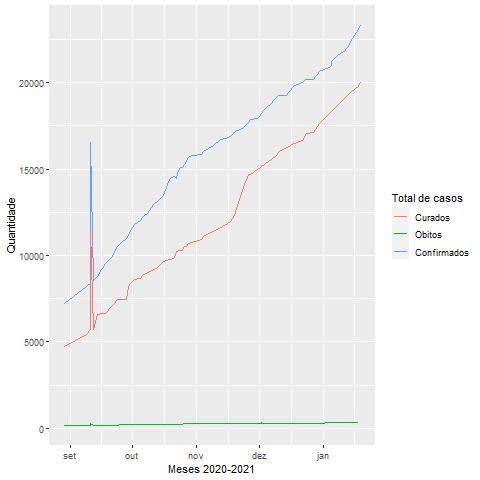
\includegraphics[width=0.35\textwidth,height=\textheight]{./graficos/infectados-curados.jpg}
\caption{Figura 2 - Infectados/Curados/Obitos}
\end{figure}

Observacoes sobre o gráfico

Nota-se diferença no número de casos em rede pública e privada,
relacionado diretamente a situação econômica, a maior parte da população
depende da rede pública de saúde.(figura 3).

\begin{figure}
\centering
\includegraphics[width=0.35\textwidth,height=\textheight]{https://miro.medium.com/max/600/1*sCJzUnDilAuvGrlllJeXKw.jpeg}
\caption{Logo do RMarkdown}
\end{figure}

Observacoes sobre o gráfico

Analisando os dados das mortes provocadas pelo coronavírus vemos neste
gráfico (figura 4) o número entre homens e mulheres que foram
contaminados, tendo como resultado um maior contágio entre homens.

\begin{figure}
\centering
\includegraphics[width=0.35\textwidth,height=\textheight]{https://miro.medium.com/max/600/1*sCJzUnDilAuvGrlllJeXKw.jpeg}
\caption{Logo do RMarkdown}
\end{figure}

Observacoes sobre o gráfico

Em relação às comorbidades, as mais comuns estão relacionadas a doenças
e tratamentos de doenças que afetam os sistemas imunológico,
respiratório, renal, cardíaco e neural.(figura 5).

\begin{figure}
\centering
\includegraphics[width=0.35\textwidth,height=\textheight]{https://miro.medium.com/max/600/1*sCJzUnDilAuvGrlllJeXKw.jpeg}
\caption{Logo do RMarkdown}
\end{figure}

Observacoes sobre o gráfico

A idade também foi bastante relevante para análise dos dados, segundo o
gráfico (figura 6) de óbitos por idade entende-se que a população idosa
é mais suscetível ao agravamento da doença.

\begin{figure}
\centering
\includegraphics[width=0.35\textwidth,height=\textheight]{https://miro.medium.com/max/600/1*sCJzUnDilAuvGrlllJeXKw.jpeg}
\caption{Logo do RMarkdown}
\end{figure}

Observacoes sobre o gráfico

\hypertarget{conclusuxe3o}{%
\subsection{Conclusão}\label{conclusuxe3o}}

Por fim, conclui-se que apesar da baixa letalidade do vírus Sars-CoV-2
há um grande número de óbitos pela facilidade de contágio e banalização
da pandemia e suas medidas de segurança.

Tendo em vista o número de casos ao longo dos meses, os dados de
internações na rede pública e privada, e o número de leitos sendo
inversamente proporcional ao número de infectados internados, podemos
deduzir que as populações mais pobres que dependem da rede pública são
as principais vítimas após o colapso do sistema de saúde pública.

As características mais comuns nos pacientes levados a óbito foram a
idade avançada, homens, comorbidades cujas doenças ou tratamento de
doenças que prejudicam os sistemas: imunológico, respiratório, renal e
cardíaco.

\hypertarget{bibliografia}{%
\subsection{Bibliografia}\label{bibliografia}}

(\url{https://covid.saude.gov.br/})

(\url{https://www.who.int/docs/default-source/ncds/un-interagency-task-force-on-ncds/uniatf-policy-brief-ncds-and-covid-030920-poster.pdf?ua=1})

(\url{https://www.bbc.com/portuguese/internacional-51674894})

(\url{https://www2.bauru.sp.gov.br/coronavirus/})

(\url{https://www.jcnet.com.br/})

\end{document}
